\documentclass[aspectratio=169,10pt]{beamer}

\usetheme{Madrid}
\usecolortheme{default}
\usepackage{amsmath,amssymb,bm}
\usepackage{booktabs}
\usepackage{array}
\usepackage{listings}
\usepackage{tikz}
\usetikzlibrary{arrows.meta,positioning,calc,fit,shapes.geometric}

\definecolor{JaxBlue}{HTML}{1261A0}
\definecolor{JaxTeal}{HTML}{138A8A}
\definecolor{JaxOrange}{HTML}{E07A1F}
\definecolor{JaxGreen}{HTML}{2E8B57}
\definecolor{JaxRed}{HTML}{B64040}
\definecolor{SoftBlue}{HTML}{EAF3FA}
\definecolor{SoftGray}{HTML}{F3F5F7}
\definecolor{CodeBg}{HTML}{F7F7F7}

\setbeamercolor{structure}{fg=JaxBlue}
\setbeamercolor{frametitle}{bg=JaxBlue,fg=white}
\setbeamercolor{title}{fg=white,bg=JaxBlue}
\setbeamercolor{subtitle}{fg=white}
\setbeamercolor{block title}{bg=JaxBlue!88,fg=white}
\setbeamercolor{block body}{bg=SoftBlue}
\setbeamercolor{alerted text}{fg=JaxRed}
\setbeamertemplate{navigation symbols}{}
\setbeamertemplate{footline}{%
  \leavevmode\hbox{%
  \begin{beamercolorbox}[wd=.78\paperwidth,ht=2.5ex,dp=1.1ex,leftskip=1em]{author in head/foot}%
    JaxCont technical presentation
  \end{beamercolorbox}%
  \begin{beamercolorbox}[wd=.22\paperwidth,ht=2.5ex,dp=1.1ex,rightskip=1em plus1fil]{date in head/foot}%
    \insertframenumber{} / \inserttotalframenumber
  \end{beamercolorbox}}}

\lstset{
  basicstyle=\ttfamily\scriptsize,
  backgroundcolor=\color{CodeBg},
  frame=single,
  rulecolor=\color{black!20},
  keywordstyle=\color{JaxBlue}\bfseries,
  commentstyle=\color{JaxGreen!80!black},
  stringstyle=\color{JaxOrange!90!black},
  showstringspaces=false,
  columns=fullflexible,
  keepspaces=true,
  breaklines=true,
  language=Python
}

\newcommand{\state}{\bm{u}}
\newcommand{\tangent}{\bm{t}}
\newcommand{\R}{\mathbb{R}}
\newcommand{\good}{\textcolor{JaxGreen}{\bfseries advantage}}
\newcommand{\limit}{\textcolor{JaxRed}{\bfseries limitation}}

\title{JaxCont Technical Presentation}
\subtitle{A beginner-friendly guide to continuation, implementation, and research applications}
\author{JaxCont}
\date{Living technical guide}

\begin{document}

\begin{frame}
  \titlepage
\end{frame}

\begin{frame}{What you should be able to explain afterwards}
\begin{enumerate}
  \item What a continuation method computes---and why it is not time integration.
  \item Why natural parameter continuation fails at a fold.
  \item How pseudo-arclength prediction and correction pass a fold.
  \item How JaxCont turns the mathematics into a compiled numerical workflow.
  \item What fixed buffers, \texttt{lax.while\_loop}, JIT and \texttt{vmap} contribute.
  \item How to plan, run, validate, and interpret a continuation study.
\end{enumerate}
\begin{alertblock}{Important naming clarification}
The function contains ``scan'' in its name, but its outer loop is currently
implemented with \texttt{jax.lax.while\_loop}, not \texttt{jax.lax.scan}.
\end{alertblock}
\end{frame}

\begin{frame}{The story in one picture}
\centering
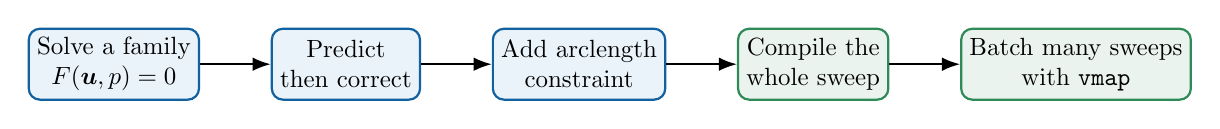
\begin{tikzpicture}[scale=.90,transform shape,node distance=8mm and 10mm,>=Latex,
 box/.style={rounded corners,draw=JaxBlue,thick,fill=SoftBlue,minimum height=10mm,align=center},
 fast/.style={rounded corners,draw=JaxGreen,thick,fill=JaxGreen!10,minimum height=10mm,align=center}]
\node[box] (math) {Solve a family\\$F(\state,p)=0$};
\node[box,right=of math] (pc) {Predict\\then correct};
\node[box,right=of pc] (palc) {Add arclength\\constraint};
\node[fast,right=of palc] (jax) {Compile the\\whole sweep};
\node[fast,right=of jax] (batch) {Batch many sweeps\\with \texttt{vmap}};
\draw[->,thick] (math)--(pc);
\draw[->,thick] (pc)--(palc);
\draw[->,thick] (palc)--(jax);
\draw[->,thick] (jax)--(batch);
\end{tikzpicture}
\vspace{8mm}
\begin{columns}[T]
\column{.48\textwidth}
\begin{block}{Numerical idea}
Reparameterize the curve by distance along the curve, not by the physical parameter alone.
\end{block}
\column{.48\textwidth}
\begin{block}{Computational idea}
Express the complete bounded algorithm as array operations that XLA can compile as one program.
\end{block}
\end{columns}
\end{frame}

\section{Continuation fundamentals}

\begin{frame}{What problem are we solving?}
Suppose a model has state $\state\in\R^n$ and parameter $p\in\R$:
\[
  \dot{\state}=F(\state,p).
\]
An equilibrium satisfies
\[
  F(\state,p)=0.
\]
\begin{columns}[T]
\column{.48\textwidth}
\begin{block}{A root solve}
Given one fixed $p$, find one $\state$ satisfying $F=0$.
\end{block}
\column{.48\textwidth}
\begin{block}{Continuation}
Follow a connected curve of pairs $(\state,p)$ satisfying $F=0$.
\end{block}
\end{columns}
\vspace{4mm}
\begin{alertblock}{Not simulation}
Continuation does not integrate $\dot{\state}$ forward in physical time. It moves along a geometric solution branch in the augmented $(\state,p)$ space.
\end{alertblock}
\end{frame}

\begin{frame}{A branch is a curve of solutions}
\centering
\begin{tikzpicture}[x=1.45cm,y=1.05cm,>=Latex]
  \draw[->] (-3.3,0)--(3.3,0) node[right] {$p$};
  \draw[->] (0,-2.7)--(0,2.7) node[above] {$u$};
  \draw[JaxBlue,very thick,smooth,domain=-2.1:2.1,samples=100]
      plot ({\x^3/3-\x},{\x});
  \foreach \x in {-1.8,-1.3,-.8,-.3,.2,.7,1.2,1.7}
    \fill[JaxOrange] ({\x^3/3-\x},{\x}) circle (1.6pt);
  \node[align=left,anchor=west] at (1.4,2.0) {Each dot is a pair\\$(u,p)$ with $F(u,p)=0$};
\end{tikzpicture}
\vspace{-2mm}
\[
F(u,p)=p+u-u^3/3=0.
\]
The output is an ordered sample of this curve, not an explicit function $u(p)$ everywhere.
\end{frame}

\begin{frame}{Why ordinary root solving is not enough}
At step $k$ we know a solution $(\state_k,p_k)$. We want a nearby one.
\begin{enumerate}
  \item Guess a nearby point: the \alert{predictor}.
  \item Solve equations to return to the exact branch: the \alert{corrector}.
  \item Accept or reject the point and choose the next step size.
\end{enumerate}
\begin{block}{Why reuse the previous solution?}
Nearby points on a smooth branch are close. The previous state is an excellent initial guess for Newton's method, so continuation is usually much cheaper than solving every parameter value from scratch.
\end{block}
\begin{alertblock}{But near a fold}
The parameter ceases to be a good coordinate. The same $p$ can correspond to several states, and $d\state/dp$ can become unbounded.
\end{alertblock}
\end{frame}

\begin{frame}{The Jacobian tells us local sensitivity}
Differentiate the equilibrium equation along a branch:
\[
  F(\state(p),p)=0
  \quad\Longrightarrow\quad
  F_{\state}\frac{d\state}{dp}+F_p=0.
\]
If $F_{\state}$ is invertible,
\[
  \frac{d\state}{dp}=-F_{\state}^{-1}F_p.
\]
\begin{columns}[T]
\column{.48\textwidth}
\begin{block}{Regular point}
$F_{\state}$ is nonsingular. State changes smoothly as $p$ changes.
\end{block}
\column{.48\textwidth}
\begin{alertblock}{Fold point}
$F_{\state}$ has a zero eigenvalue. The inverse formula breaks down.
\end{alertblock}
\end{columns}
JaxCont obtains both $F_{\state}$ and $F_p$ with \texttt{jax.jacfwd}; no hand-coded finite difference is needed.
\end{frame}

\begin{frame}{A fold: the parameter turns around}
\centering
\begin{tikzpicture}[x=1.45cm,y=1.05cm,>=Latex]
  \draw[->] (-3.2,0)--(3.2,0) node[right] {$p$};
  \draw[->] (0,-2.7)--(0,2.7) node[above] {$u$};
  \draw[JaxBlue,very thick,smooth,domain=-2.1:2.1,samples=100]
      plot ({\x^3/3-\x},{\x});
  \fill[JaxRed] ({2/3},{-1}) circle (3pt) node[right=2mm] {fold};
  \fill[JaxRed] ({-2/3},{1}) circle (3pt) node[left=2mm] {fold};
  \draw[JaxOrange,very thick,->] (-1.3,-1.75)..controls(-.1,-1.4) and (.8,-1.2)..({2/3},{-1});
  \draw[JaxOrange,very thick,->] ({2/3},{-1})..controls(.5,-.6) and (.1,-.2)..(-.2,.3);
\end{tikzpicture}
\begin{itemize}
  \item The physical parameter $p$ increases, stops, then decreases.
  \item The branch itself remains smooth in $(u,p)$ space.
  \item The remedy is to parameterize by progress \emph{along the curve}.
\end{itemize}
\end{frame}

\section{Natural and pseudo-arclength methods}

\begin{frame}{Natural parameter continuation}
Natural continuation treats $p$ as the independent coordinate.
\[
  p_{\mathrm{pred}}=p_k+\operatorname{sign}(p_{\mathrm{end}}-p_k)\,\Delta s,
  \qquad \state_{\mathrm{pred}}=\state_k.
\]
Then Newton solves only
\[
  F(\state,p_{\mathrm{pred}})=0
\]
with $p_{\mathrm{pred}}$ fixed.
\begin{block}{Advantages}
Simple, cheap, intuitive, and effective on branches that are single-valued as $\state(p)$.
\end{block}
\begin{alertblock}{Limitation}
At a fold, Newton must invert $F_{\state}$, which becomes singular. Shrinking the step can approach the fold, but it cannot change this geometry.
\end{alertblock}
\end{frame}

\begin{frame}{Why natural continuation stalls at a fold}
\centering
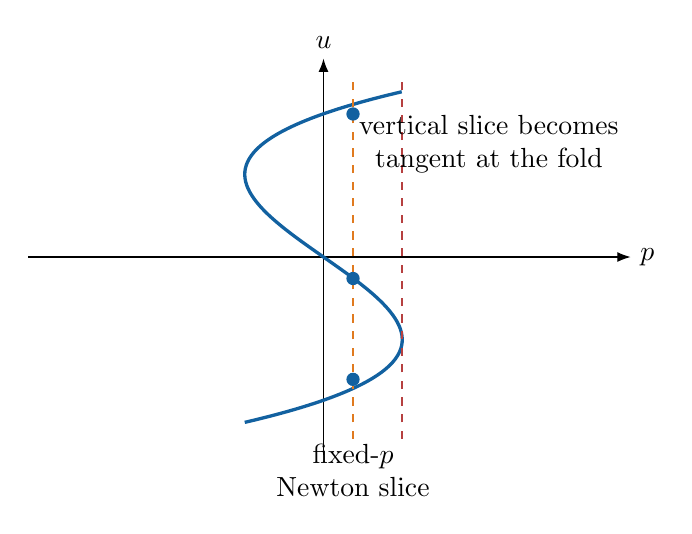
\begin{tikzpicture}[x=1.5cm,y=1.05cm,>=Latex]
  \draw[->] (-2.5,0)--(2.6,0) node[right] {$p$};
  \draw[->] (0,-2.4)--(0,2.4) node[above] {$u$};
  \draw[JaxBlue,very thick,smooth,domain=-2:2,samples=100]
      plot ({\x^3/3-\x},{\x});
  \draw[JaxOrange,dashed,thick] (.25,-2.2)--(.25,2.2);
  \fill[JaxBlue] (.25,-1.48) circle (2.4pt);
  \fill[JaxBlue] (.25,-.26) circle (2.4pt);
  \fill[JaxBlue] (.25,1.73) circle (2.4pt);
  \draw[JaxRed,dashed,thick] ({2/3},-2.2)--({2/3},2.2);
  \node[align=center,anchor=north] at (.25,-2.15) {fixed-$p$\\Newton slice};
  \node[align=center,anchor=south] at (1.4,.9) {vertical slice becomes\\tangent at the fold};
\end{tikzpicture}
\begin{itemize}
  \item Multiple roots may exist for one $p$.
  \item The fixed-$p$ slice touches the branch instead of crossing it transversally.
  \item Newton loses a unique local correction direction.
\end{itemize}
\end{frame}

\begin{frame}{Pseudo-arclength continuation: the key idea}
Introduce an artificial curve coordinate $s$. Seek
\[
  (\state(s),p(s)) \quad\text{such that}\quad F(\state(s),p(s))=0.
\]
Use the previous unit tangent
\[
  \tangent_k=(\dot{\state}_k,\dot p_k),
  \qquad \|\tangent_k\|_2=1,
\]
to predict a new point:
\[
  (\state_{\mathrm{pred}},p_{\mathrm{pred}})
  =(\state_k,p_k)+\Delta s\,\tangent_k.
\]
\begin{block}{The conceptual change}
Both the state and the physical parameter are now unknowns during correction. The algorithm can naturally allow $p$ to turn around.
\end{block}
\end{frame}

\begin{frame}{Geometry of predictor and corrector}
\centering
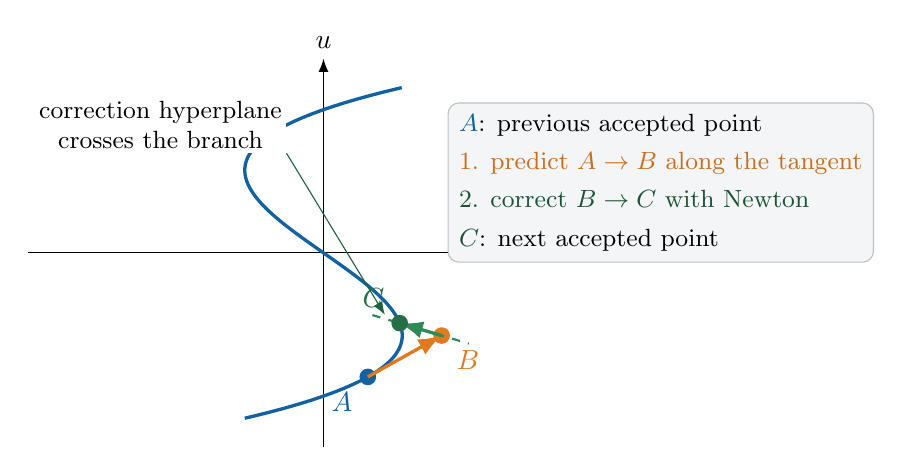
\begin{tikzpicture}[x=1.5cm,y=1.05cm,>=Latex,
  labelbox/.style={fill=white,inner sep=1.5pt,font=\small}]
  \draw[->] (-2.5,0)--(2.8,0) node[right] {$p$};
  \draw[->] (0,-2.35)--(0,2.35) node[above] {$u$};
  \draw[JaxBlue,very thick,smooth,domain=-2:2,samples=100]
      plot ({\x^3/3-\x},{\x});
  \coordinate (old) at (.375,-1.50);
  \coordinate (pred) at (1.00,-1.00);
  \coordinate (new) at (.645,-.85);

  % Short A/B/C markers keep the small correction triangle readable; the
  % explanations live in the legend at upper right.
  \fill[JaxBlue] (old) circle (3pt) node[below left=1mm] {$A$};

  \draw[JaxOrange,very thick,->] (old)--(pred);
  \fill[JaxOrange] (pred) circle (3pt) node[below right=1mm] {$B$};

  \draw[JaxGreen,dashed,thick] ($(new)!-.65!(pred)$)--($(new)!1.65!(pred)$);
  \draw[JaxGreen,very thick,->] (pred)--(new);
  \fill[JaxGreen!80!black] (new) circle (3pt) node[above left=1mm] {$C$};

  \node[draw=black!25,rounded corners,fill=SoftGray,anchor=north west,
        align=left,font=\small,inner sep=4pt] at (1.05,1.82) {
    \textcolor{JaxBlue}{$A$}: previous accepted point\\[1mm]
    \textcolor{JaxOrange!90!black}{1. predict $A\rightarrow B$ along the tangent}\\[1mm]
    \textcolor{JaxGreen!60!black}{2. correct $B\rightarrow C$ with Newton}\\[1mm]
    \textcolor{JaxGreen!60!black}{$C$}: next accepted point};

  \node[labelbox,align=center] (plane) at (-1.38,1.55)
      {correction hyperplane\\crosses the branch};
  \draw[JaxGreen!70!black,->,thin] (plane.south east)--(.52,-.75);
\end{tikzpicture}
\end{frame}

\begin{frame}{The extra pseudo-arclength equation}
The corrector solves $n+1$ equations for the $n+1$ unknowns $(\state,p)$:
\[
\begin{cases}
F(\state,p)=0,\\[1mm]
g(\state,p)=
(\state-\state_k)^T\dot{\state}_k
+(p-p_k)\dot p_k-\Delta s=0.
\end{cases}
\]
\begin{itemize}
  \item $F=0$ places the point on the solution branch.
  \item $g=0$ places it on a hyperplane normal to the previous tangent.
  \item Their intersection selects one nearby point, even at a fold.
\end{itemize}
\begin{block}{Why ``pseudo''?}
$\Delta s$ approximates geometric arclength locally; it is not the exact integral of speed along the curve.
\end{block}
\end{frame}

\begin{frame}{How JaxCont computes the tangent}
The tangent lies in the null space of the total derivative:
\[
  \begin{bmatrix}F_{\state} & F_p\end{bmatrix}
  \begin{bmatrix}\dot{\state}\\ \dot p\end{bmatrix}=0.
\]
JaxCont selects and orients a unique tangent with the bordered system
\[
\begin{bmatrix}
F_{\state} & F_p\\
\tangent_{k-1}^{T}
\end{bmatrix}
\tangent_k=
\begin{bmatrix}\bm{0}\\1\end{bmatrix},
\qquad
\tangent_k\leftarrow\frac{\tangent_k}{\|\tangent_k\|_2}.
\]
If $\tangent_k^T\tangent_{k-1}<0$, its sign is flipped.
\begin{block}{Why align signs?}
Both $\tangent$ and $-\tangent$ solve the null-vector equation. Sign alignment prevents the continuation direction from alternating randomly.
\end{block}
\end{frame}

\begin{frame}{The bordered Newton correction}
One Newton iteration solves
\[
\underbrace{\begin{bmatrix}
F_{\state} & F_p\\
\dot{\state}_k^T & \dot p_k
\end{bmatrix}}_{\text{bordered Jacobian}}
\begin{bmatrix}\delta\state\\\delta p\end{bmatrix}
=-
\begin{bmatrix}F(\state,p)\\g(\state,p)\end{bmatrix}.
\]
Then update
\[
  \state\leftarrow\state+\delta\state,
  \qquad p\leftarrow p+\delta p.
\]
\begin{alertblock}{The crucial robustness point}
At a fold, $F_{\state}$ alone is singular, but the full bordered matrix can remain nonsingular. JaxCont solves this full system rather than eliminating through $F_{\state}^{-1}$.
\end{alertblock}
\end{frame}

\begin{frame}{One pseudo-arclength step}
\begin{enumerate}
  \item Start with accepted $(\state_k,p_k)$, tangent $\tangent_k$, and step $\Delta s$.
  \item Predict $(\state,p)=(\state_k,p_k)+\Delta s\,\tangent_k$.
  \item Newton-correct the augmented system $(F,g)=0$.
  \item If finite and converged: store the point and compute $\tangent_{k+1}$.
  \item If rejected: keep the old point and reduce $\Delta s$.
  \item Stop at the parameter target, minimum-step failure, non-finite state, or step budget.
\end{enumerate}
\begin{block}{State machine view}
The entire algorithm is a bounded transition from one immutable carry state to the next. That formulation is exactly what JAX control-flow primitives need.
\end{block}
\end{frame}

\begin{frame}{Adaptive step size in the branch implementation}
The continuation engine uses Newton effort as a difficulty signal:
\begin{center}
\begin{tabular}{lll}
\toprule
Outcome & Rule & Interpretation\\
\midrule
Converged in $<3$ iterations & $\Delta s\leftarrow1.5\Delta s$ & branch is easy\\
Converged in $3$--$6$ & unchanged & suitable step\\
Converged in $>6$ & $\Delta s\leftarrow0.8\Delta s$ & branch is difficult\\
Failed & $\Delta s\leftarrow0.5\Delta s$ & retry more cautiously\\
\bottomrule
\end{tabular}
\end{center}
Finally clip to $[\Delta s_{\min},\Delta s_{\max}]$.
\begin{alertblock}{Subtle implementation trade-off}
A failed attempt consumes one outer-loop iteration but does not consume an output slot. Therefore \texttt{max\_steps} should include retry headroom.
\end{alertblock}
\end{frame}

\section{How JaxCont implements the methods}

\begin{frame}{What does \texttt{pseudo\_arclength\_scan} mean?}
\begin{columns}[T]
\column{.47\textwidth}
\begin{block}{Pseudo-arclength}
The numerical method: tangent prediction plus augmented Newton correction.
\end{block}
\column{.47\textwidth}
\begin{block}{Scan engine}
The implementation style: execute the whole bounded branch sweep inside one compiled functional loop.
\end{block}
\end{columns}
\vspace{5mm}
\begin{alertblock}{Do not say this}
``JaxCont uses the \texttt{lax.scan} algorithm for arclength continuation.''
\end{alertblock}
\begin{block}{Say this instead}
``JaxCont's scan engine packages the complete continuation sweep into a JIT-compiled \texttt{lax.while\_loop}. The mathematical algorithm inside that loop is pseudo-arclength continuation.''
\end{block}
\end{frame}

\begin{frame}{Choosing a continuation method}
\begin{columns}[T]
\column{.48\textwidth}
\begin{block}{Use \texttt{Natural()} when}
\begin{itemize}
  \item the branch is expected to be single-valued in $p$;
  \item folds are not part of the research question;
  \item a simple reference calculation is useful.
\end{itemize}
\end{block}
\column{.48\textwidth}
\begin{block}{Use \texttt{PseudoArclength()} when}
\begin{itemize}
  \item folds or hysteresis may occur;
  \item the branch can turn in the parameter;
  \item robust branch following matters more than the smallest linear system.
\end{itemize}
\end{block}
\end{columns}
\vspace{4mm}
\begin{alertblock}{Practical default}
For exploratory bifurcation analysis, pseudo-arclength is usually the safer
starting choice. Natural continuation remains useful for simple monotone
branches and for learning the predictor--corrector idea.
\end{alertblock}
\end{frame}

\begin{frame}{From a user request to a computed branch}
\centering
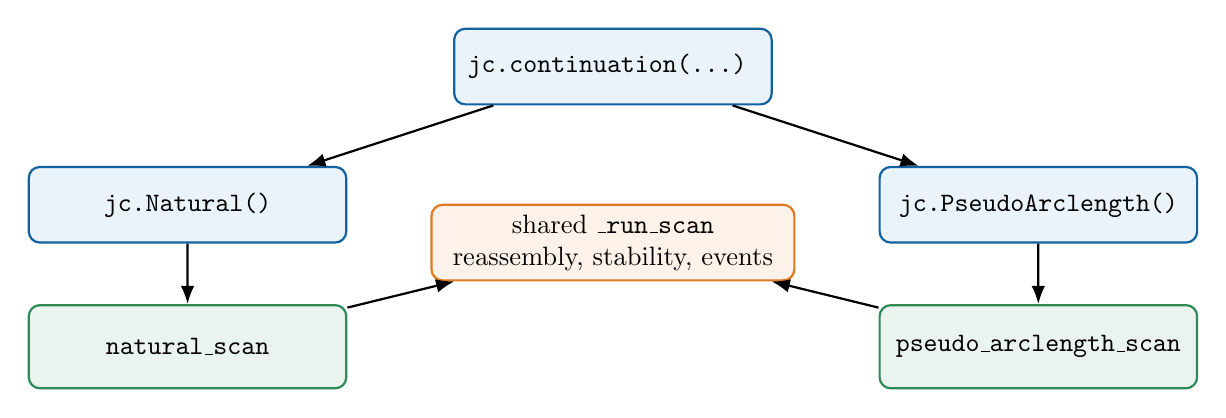
\begin{tikzpicture}[scale=.96,transform shape,node distance=8mm and 14mm,>=Latex,
 api/.style={rounded corners,draw=JaxBlue,thick,fill=SoftBlue,minimum width=42mm,minimum height=10mm,align=center},
 eng/.style={rounded corners,draw=JaxGreen,thick,fill=JaxGreen!10,minimum width=42mm,minimum height=11mm,align=center},
 shared/.style={rounded corners,draw=JaxOrange,thick,fill=JaxOrange!10,minimum width=48mm,minimum height=10mm,align=center}]
\node[api] (call) {\texttt{jc.continuation(...)} };
\node[api,below left=of call] (nat) {\texttt{jc.Natural()}};
\node[api,below right=of call] (palc) {\texttt{jc.PseudoArclength()}};
\node[eng,below=of nat] (ns) {\texttt{natural\_scan}};
\node[eng,below=of palc] (ps) {\texttt{pseudo\_arclength\_scan}};
\node[shared,below=13mm of call] (run) {shared \texttt{\_run\_scan}\\reassembly, stability, events};
\draw[->,thick] (call)--(nat); \draw[->,thick] (call)--(palc);
\draw[->,thick] (nat)--(ns); \draw[->,thick] (palc)--(ps);
\draw[->,thick] (ns)--(run); \draw[->,thick] (ps)--(run);
\end{tikzpicture}
\vspace{3mm}
Both methods return the same fixed-shape \texttt{ScanResult}. This gives
plotting, stability analysis, and event detection one predictable input format.
\end{frame}

\begin{frame}[fragile]{The public API stays simple}
\begin{lstlisting}
import jaxcont as jc

problem = jc.bif_problem(f, u0=u0, p0=p0, args=args)
settings = jc.ContinuationPar(
    ds=0.02, ds_min=1e-5, ds_max=0.1,
    max_steps=300, newton_tol=1e-6,
    compute_stability=True,
)

result = jc.continuation(
    problem,
    jc.PseudoArclength(),
    p_span=(p0, p_end),
    settings=settings,
    events=[jc.Fold(), jc.Hopf()],
)
\end{lstlisting}
The algorithm object selects the numerical engine; shared result assembly keeps plotting, stability and event consumers independent of the engine.
\end{frame}

\begin{frame}{Important start-point semantics}
\begin{block}{The pair that actually starts continuation}
\[
  (\state_0,p_{\mathrm{start}})=(\texttt{problem.u0},\;\texttt{p\_span[0]}).
\]
The first value of \texttt{p\_span} is a literal starting parameter; it is not
silently replaced by \texttt{problem.p0}.
\end{block}
\begin{itemize}
  \item Supply an initial state satisfying $F(\state_0,\texttt{p\_span[0]})\approx0$.
  \item \texttt{problem.p0} records the problem's reference/default parameter, but does not override the continuation interval.
  \item This became explicit while migrating the final gallery examples from the removed object-oriented API.
\end{itemize}
\begin{alertblock}{Common failure mode}
Pairing an equilibrium computed at \texttt{problem.p0} with a different
\texttt{p\_span[0]} can make the first correction fail or follow the wrong branch.
\end{alertblock}
\end{frame}

\begin{frame}{What is carried through the compiled loop?}
\begin{center}
\begin{tabular}{ll}
\toprule
Carry field & Meaning\\
\midrule
$\state,p$ & last accepted solution\\
$\tangent$ & last accepted tangent (pseudo-arclength only)\\
$\Delta s$ & current positive step magnitude\\
\texttt{idx} & number of accepted steps / next write position\\
\texttt{stop} & compiled termination flag\\
$P,Q,T,C,D$ & state, parameter, tangent, convergence, step-size buffers\\
\bottomrule
\end{tabular}
\end{center}
Each body call returns a completely new carry. There is no Python object mutation inside the compiled numerical kernel.
\end{frame}

\begin{frame}{The common \texttt{ScanResult}}
For state dimension $n$ and maximum $M$ steps:
\begin{center}
\begin{tabular}{lll}
\toprule
Field & Shape & Content\\
\midrule
\texttt{states} & $(M+1,n)$ & accepted states plus unused slots\\
\texttt{params} & $(M+1)$ & parameter values\\
\texttt{tangents} & $(M+1,n+1)$ & PALC tangents; zeros for natural\\
\texttt{converged} & $(M+1)$ & accepted-slot flags\\
\texttt{ds} & $(M+1)$ & step used to reach each point\\
\texttt{n\_valid} & scalar & real points occupy \texttt{[:n\_valid]}\\
\bottomrule
\end{tabular}
\end{center}
\begin{block}{Why share the shape?}
One result type allows both engines to use the same eager/traced reassembly path without shape-dependent branching.
\end{block}
\end{frame}

\begin{frame}{Safe and bounded termination}
The outer loop stops when any condition becomes true:
\begin{enumerate}
  \item at most \texttt{max\_steps} attempts have run;
  \item the accepted parameter reaches the requested endpoint;
  \item a failed step shrinks to \texttt{ds\_min};
  \item a state becomes non-finite.
\end{enumerate}
The inner Newton loop stops at convergence, non-finite residual, or \texttt{max\_iter}.
\begin{block}{Why this matters}
Bounded loops and explicit finite-value guards prevent a compiled computation from hanging forever on a pathological branch.
\end{block}
\end{frame}

\section{How it is made fast}

\begin{frame}{Why compile the complete continuation loop?}
Small systems perform many tiny operations per point:
\[
\text{Python step}\to F\to \text{Jacobian}\to\text{solve}\to F\to\cdots
\]
Each arrow can cause Python orchestration and device dispatch.
\begin{block}{Optimization target}
Place prediction, Newton correction, step adaptation, buffer writes, and
termination inside one compiled program. The mathematics remains sequential,
but the device executes the sequence without returning to Python at every step.
\end{block}
\begin{alertblock}{What this does not mean}
Compilation does not improve an ill-conditioned model or repair a poor initial
equilibrium. It reduces execution overhead; numerical validity still depends on
the continuation setup.
\end{alertblock}
\end{frame}

\begin{frame}{Whole-loop JIT}
\centering
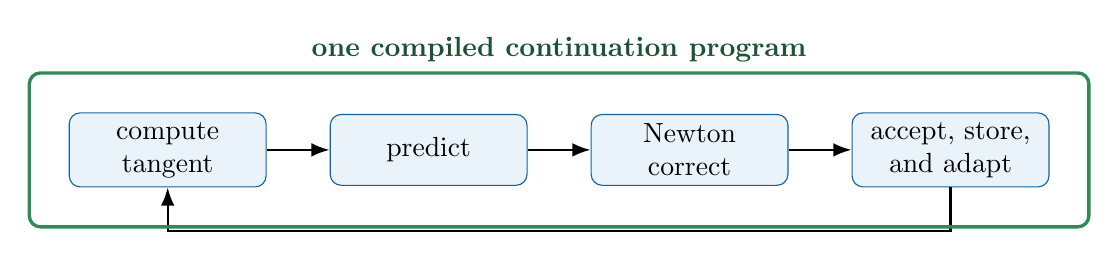
\begin{tikzpicture}[node distance=6mm and 8mm,>=Latex,
 stage/.style={draw=JaxBlue,fill=SoftBlue,rounded corners,minimum width=25mm,
              minimum height=9mm,align=center},
 boundary/.style={draw=JaxGreen,very thick,rounded corners,inner sep=5mm}]
\node[stage] (tan) {compute\\tangent};
\node[stage,right=of tan] (pred) {predict};
\node[stage,right=of pred] (corr) {Newton\\correct};
\node[stage,right=of corr] (adapt) {accept, store,\\and adapt};
\draw[->,thick] (tan)--(pred);
\draw[->,thick] (pred)--(corr);
\draw[->,thick] (corr)--(adapt);
\draw[->,thick] (adapt.south) -- ++(0,-.55) -| (tan.south);
\node[boundary,fit=(tan)(pred)(corr)(adapt),
      label={[text=JaxGreen!60!black,font=\bfseries]above:one compiled continuation program}] {};
\end{tikzpicture}
\vspace{5mm}
\begin{block}{The JIT boundary}
\small
\texttt{@partial(jax.jit, static\_argnums=(0, 8))} wraps the full engine.
The model function and buffer length are static, so compatible later calls
reuse the compiled executable.
\end{block}
\end{frame}

\begin{frame}{Compilation versus execution}
\begin{enumerate}
  \item \textbf{Trace:} JAX observes array operations and control-flow primitives.
  \item \textbf{Compile:} XLA optimizes a device program for shapes/dtypes/static values.
  \item \textbf{Execute:} later compatible calls reuse the compiled program.
\end{enumerate}
\begin{columns}[T]
\column{.48\textwidth}
\begin{alertblock}{Cold call}
Includes compilation; can be slower and should not be compared directly with an already-warm Python implementation.
\end{alertblock}
\column{.48\textwidth}
\begin{block}{Warm call}
Reuses the executable; this measures steady-state throughput.
\end{block}
\end{columns}
\vspace{3mm}
Always call \texttt{block\_until\_ready()} when timing asynchronous JAX work.
\end{frame}

\begin{frame}{Static values versus traced values}
In the engine decorator, arguments 0 and 8 are static:
\begin{itemize}
  \item \texttt{f}: the Python model function defines the compiled program;
  \item \texttt{max\_steps}: determines buffer shapes.
\end{itemize}
Traced array values include $\state_0,p_0,p_{end},\Delta s$, tolerances and Newton limits.
\begin{block}{Practical consequence}
Changing array values usually reuses a compilation. Changing state shape, dtype, model function, or static step budget can trigger recompilation.
\end{block}
\begin{alertblock}{Performance rule}
Do not vary static configuration unnecessarily inside a sweep; group runs by compatible shapes and static settings.
\end{alertblock}
\end{frame}

\begin{frame}{Fixed-size buffers unlock transformations}
Python would normally append each accepted point to a growing list. JAX transformations require predictable array shapes.
\begin{center}
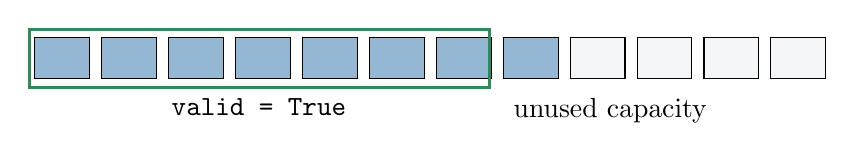
\begin{tikzpicture}[x=.85cm,y=.7cm]
\foreach \i in {0,...,11} {
  \draw[fill=SoftGray] (\i,0) rectangle +(0.82,0.75);
}
\foreach \i in {0,...,7} {
  \draw[fill=JaxBlue!45] (\i,0) rectangle +(0.82,0.75);
}
\draw[JaxGreen,very thick] (-.08,-.15) rectangle (6.8,.9);
\node[below] at (3.35,-.18) {\texttt{valid = True}};
\node[below] at (8.6,-.18) {unused capacity};
\end{tikzpicture}
\end{center}
Return all $M+1$ slots plus \texttt{n\_valid} or a boolean \texttt{valid} mask.
\begin{block}{The trade-off}
Some memory is reserved for unused points, but output shapes become compatible with JIT, batching, accelerators and PyTrees.
\end{block}
\end{frame}

\begin{frame}{Branch-free array control}
Inside traced code, Python decisions such as
\begin{center}
\texttt{if converged: append(new\_state)}
\end{center}
cannot depend on a runtime tracer. The engine uses array selection:
\[
\state_{\mathrm{next}}=\operatorname{where}
(\text{converged},\state_{\mathrm{new}},\state_{\mathrm{old}}).
\]
Likewise, the buffer write, tangent update, index advance and step-size rule use \texttt{jnp.where} and logical array operations.
\begin{block}{Strategy}
Compute candidates in a uniform program, then select the valid state with array primitives. This makes control flow traceable and device-friendly.
\end{block}
\end{frame}

\begin{frame}[fragile]{\texttt{vmap}: many branches, one batched program}
\begin{lstlisting}
def run_one(design_value):
    prob_i = problem.at(args=design_value)
    return jc.continuation(
        prob_i, jc.PseudoArclength(),
        p_span=(p0, p1), settings=settings,
    )

branches = jax.vmap(run_one)(design_values)
\end{lstlisting}
\begin{itemize}
  \item No explicit Python loop over designs.
  \item Batch axes propagate through Jacobians, linear solves and buffers.
  \item Particularly valuable on GPUs and for parameter ensembles.
\end{itemize}
\begin{alertblock}{Shape requirement}
Every batched run returns the same buffer shape; each run's \texttt{valid} mask identifies its actual branch length.
\end{alertblock}
\end{frame}

\begin{frame}{Stability is a vectorized post-pass}
For equilibria, local stability comes from eigenvalues of
\[
  J_k=F_{\state}(\state_k,p_k).
\]
JaxCont maps one eigenvalue calculation over stored branch points:
\[
  \{(\state_k,p_k)\}_{k=0}^{M}
  \xrightarrow{\texttt{jax.vmap}}
  \{\operatorname{eigvals}(J_k)\}_{k=0}^{M}.
\]
An equilibrium is marked stable if every eigenvalue has negative real part.
\begin{block}{Why outside the sequential loop?}
Continuation steps depend on previous steps, but stability evaluations of already stored points are independent and therefore naturally parallel.
\end{block}
\end{frame}

\begin{frame}{Automatic differentiation is used in two roles}
\begin{enumerate}
  \item \textbf{Inside the solver:} \texttt{jacfwd} computes $F_{\state}$ and $F_p$ for tangents and Newton corrections.
  \item \textbf{Around the solver:} forward-mode differentiation can propagate through the whole \texttt{while\_loop} sweep.
\end{enumerate}
\begin{block}{Why forward mode here?}
Continuation often differentiates outputs with respect to a small number of design parameters; forward mode is structurally compatible with \texttt{lax.while\_loop}.
\end{block}
\begin{alertblock}{Not magic}
Automatic differentiation produces derivatives of the implemented discrete algorithm. Conditioning, convergence and branch identity still determine whether those derivatives are scientifically meaningful.
\end{alertblock}
\end{frame}

\begin{frame}{Reverse mode and the differentiable-fold strategy}
Reverse-mode differentiation through dynamic \texttt{lax.while\_loop} is not generally supported in the desired way.
JaxCont handles fold-location gradients separately:
\begin{enumerate}
  \item Solve an extended fold system $G(z,\theta)=0$.
  \item Define a custom reverse rule using the implicit function theorem.
  \item Solve an adjoint linear system instead of backpropagating through every Newton iteration.
\end{enumerate}
\[
  \frac{dz^*}{d\theta}=-G_z^{-1}G_{\theta}.
\]
\begin{block}{Distinction to remember}
The scan engine provides the branch; the custom-VJP fold solver provides efficient reverse-mode gradients of a selected bifurcation point.
\end{block}
\end{frame}

\begin{frame}{The eager and traced result paths}
\begin{columns}[T]
\column{.48\textwidth}
\begin{block}{Eager call}
Convert \texttt{n\_valid} to a Python integer, trim buffers, run existing event detection, and build convenient Python metadata.
\end{block}
\column{.48\textwidth}
\begin{block}{Inside JIT / \texttt{vmap}}
The length is a tracer. Return full buffers and a \texttt{valid} mask; avoid Python lists, \texttt{float()}, sorting and variable-length trimming.
\end{block}
\end{columns}
\vspace{5mm}
\begin{alertblock}{Current boundary}
\texttt{events=[Fold(), Hopf()]} is not supported inside \texttt{jax.vmap}/\texttt{jax.jit}; the legacy detector uses Python-level control flow. Branch and stability data are transformation-safe.
\end{alertblock}
\end{frame}

\begin{frame}{When acceleration helps a research study}
\begin{itemize}
  \item Repeating the same branch calculation for many parameter sets.
  \item Screening uncertain parameters or candidate model designs.
  \item Differentiating a selected output with respect to a few design variables.
  \item Running independent continuation problems as a \texttt{vmap} batch.
  \item Reusing one compiled program for calls with compatible shapes and settings.
\end{itemize}
\begin{alertblock}{Measure the workload you actually care about}
Record compilation time and warm execution time separately. Document hardware,
precision, model dimension, \texttt{max\_steps}, branch length, and batch size;
these determine whether acceleration is scientifically useful.
\end{alertblock}
\end{frame}

\begin{frame}{Computational limits to plan for}
\begin{itemize}
  \item Dense Jacobians and dense $(n+1)\times(n+1)$ solves dominate as $n$ grows.
  \item Fixed buffers cost memory proportional to \texttt{max\_steps}.
  \item Changing static shapes/settings can cause recompilation.
  \item Event detection currently returns to Python on eager runs.
  \item The first call pays tracing and compilation cost.
  \item A sequential branch cannot parallelize across its own steps; batching parallelizes \emph{across branches}.
\end{itemize}
\begin{block}{Planning implication}
Estimate state dimension, number of branch points, and ensemble size before a
large study. Start with a small validated run, then increase resolution or
batch size while monitoring memory and convergence.
\end{block}
\end{frame}

\section{Research applications and workflow}

\begin{frame}{What continuation can answer}
\begin{center}
\begin{tabular}{>{\raggedright\arraybackslash}p{.29\textwidth}
                >{\raggedright\arraybackslash}p{.59\textwidth}}
\toprule
Research question & Continuation output\\
\midrule
Where do equilibria exist? & A connected branch of steady states over a parameter range.\\
Where can abrupt transitions occur? & Fold candidates and multistable parameter regions.\\
When does an equilibrium lose stability? & Stability changes and candidate local bifurcations.\\
How robust is a conclusion? & Batches of branches over uncertain parameters or model variants.\\
How does a threshold move? & Sensitivity of a selected, well-defined bifurcation point.\\
\bottomrule
\end{tabular}
\end{center}
\begin{alertblock}{Interpretation boundary}
A bifurcation diagram describes model solutions and their local stability. It
does not by itself establish causality, fit parameters, or validate the model
against observations.
\end{alertblock}
\end{frame}

\begin{frame}{A beginner-friendly research workflow}
\begin{enumerate}
  \item State the scientific question and choose one continuation parameter.
  \item Implement a deterministic, smooth residual $F(\state,p)$.
  \item Find one equilibrium and verify $\|F(\state_0,p_0)\|$ is small.
  \item Run a short continuation with conservative settings.
  \item Inspect convergence, branch shape, stability, and possible events.
  \item Repeat in the opposite direction or from another known equilibrium.
  \item Refine interesting regions and validate them independently.
  \item Save code, settings, precision, hardware, and diagnostic information.
\end{enumerate}
\begin{block}{Start small}
Use a reduced model or narrow parameter interval first. A trustworthy small
calculation is more valuable than a large unexplained diagram.
\end{block}
\end{frame}

\begin{frame}{How to validate a computed branch}
\begin{itemize}
  \item Check $\|F(\state_k,p_k)\|$ at accepted points, not only a success flag.
  \item Repeat with smaller and larger step-size bounds.
  \item Continue from both directions and compare overlapping branch segments.
  \item Compare simple cases with an analytic solution when one exists.
  \item Confirm important events with eigenvalues and a refined local solve.
  \item Compare selected results with simulation or another continuation tool.
  \item Test scientific conclusions under plausible parameter and model changes.
\end{itemize}
\begin{block}{Software tests and research validation are different}
Repository tests check implementation behavior. Researchers must additionally
check that their model, starting solution, parameter range, and interpretation
are appropriate for the scientific question.
\end{block}
\end{frame}

\begin{frame}{How to read the result}
\begin{itemize}
  \item Use only entries selected by \texttt{valid} or \texttt{[:n\_valid]}.
  \item Plot a scientifically meaningful state observable against $p$.
  \item Treat stability as local information about the equilibrium.
  \item Treat detected events as candidates until they are refined and checked.
  \item Inspect step sizes and residuals near sharp turns or failed regions.
  \item Keep separate branches separate; one run may not reveal every solution.
\end{itemize}
\begin{alertblock}{A missing point is not necessarily a missing solution}
Continuation can stop because of settings, conditioning, non-finite model
values, or the attempt budget. Diagnose termination before concluding that a
physical branch ends.
\end{alertblock}
\end{frame}

\begin{frame}{Current capability boundaries}
\begin{itemize}
  \item Event detection is not transformation-safe inside \texttt{jit}/\texttt{vmap}.
  \item Difficult spectra can produce ambiguous or duplicate event candidates.
  \item Dense linear algebra limits scaling to large systems.
  \item Natural continuation is intentionally unable to pass folds.
  \item Reverse-mode gradients require implicit/custom rules rather than backpropagation through the scan loop.
  \item Following equilibrium branches does not compute periodic-orbit amplitude or stability.
  \item Branch switching and discovery of disconnected branches require additional analysis.
\end{itemize}
\begin{block}{Use the tool within its scope}
JaxCont is a numerical aid for structured exploration. Combine its output with
model-specific reasoning, diagnostics, independent calculations, and domain
evidence.
\end{block}
\end{frame}

\begin{frame}{A two-minute explanation you can give}
\begin{quote}
JaxCont follows equilibria $F(u,p)=0$ as a curve. Natural continuation increments $p$ and solves for $u$, so it fails when the curve folds and $F_u$ becomes singular. Pseudo-arclength instead treats both $u$ and $p$ as unknowns, predicts along the curve tangent, and adds one geometric constraint during Newton correction. The resulting bordered system remains solvable through an ordinary fold.

The ``scan'' engine is the implementation: the complete bounded predictor--corrector sweep is expressed as a pure \texttt{lax.while\_loop} over fixed-size buffers and JIT-compiled as one XLA program. Fixed shapes and masks make the result compatible with \texttt{vmap}, so many branches can run as one batched accelerator program. Researchers still need a valid starting equilibrium, suitable settings, diagnostics, and independent validation before interpreting the branch scientifically.
\end{quote}
\end{frame}

\begin{frame}{Vocabulary checklist}
\begin{description}
  \item[Continuation] following a connected family of solutions.
  \item[Predictor] a local guess for the next branch point.
  \item[Corrector] Newton iterations that return the guess to the branch.
  \item[Fold] a regular turning point where $F_{\state}$ is singular.
  \item[Pseudo-arclength] continuation using an approximate curve-distance coordinate.
  \item[Bordered system] the Jacobian enlarged with parameter and constraint rows/columns.
  \item[JIT] trace and compile array code for later reuse.
  \item[\texttt{lax.while\_loop}] JAX's compiled, traceable dynamic loop primitive.
  \item[\texttt{vmap}] automatic batching of one function across an array axis.
  \item[PyTree] a nested data structure JAX knows how to flatten into array leaves.
\end{description}
\end{frame}

\begin{frame}{Main takeaways}
\begin{enumerate}
  \item The mathematical breakthrough is reparameterization: follow the branch by local arclength, not only by $p$.
  \item The numerical workhorse is the full bordered Newton solve, which remains regular at ordinary folds.
  \item Whole-loop compilation reduces orchestration overhead and enables reusable, batched array programs.
  \item Fixed buffers, masks and array control flow are the price of JIT/\texttt{vmap}/GPU compatibility.
  \item A useful study begins with a verified equilibrium and ends with independent validation.
  \item Fast computation does not remove numerical or scientific responsibilities.
\end{enumerate}
\end{frame}

\appendix
\section{Appendix}

\begin{frame}{Appendix: natural versus pseudo-arclength}
\small
\begin{center}
\begin{tabular}{p{.25\textwidth}p{.32\textwidth}p{.32\textwidth}}
\toprule
 & Natural & Pseudo-arclength\\
\midrule
Unknown during correction & $\state$ & $(\state,p)$\\
Fixed quantity & predicted $p$ & approximate distance from previous point\\
Newton matrix & $F_{\state}$ & $\begin{bmatrix}F_{\state}&F_p\\\dot\state^T&\dot p\end{bmatrix}$\\[3mm]
At ordinary fold & singular / stalls & usually remains regular\\
Cost per Newton step & $n\times n$ solve & $(n+1)\times(n+1)$ solve\\
JaxCont engine & \texttt{natural\_scan} & \texttt{pseudo\_arclength\_scan}\\
\bottomrule
\end{tabular}
\end{center}
\end{frame}

\begin{frame}{Appendix: scalar cubic fold derivation}
For
\[
F(u,p)=p+u-u^3/3=0,
\]
the branch can be written
\[
p(u)=u^3/3-u.
\]
Folds occur when
\[
\frac{dp}{du}=u^2-1=0
\quad\Longrightarrow\quad u=\pm1.
\]
Therefore
\[
(u,p)=(-1,2/3),\qquad(1,-2/3).
\]
Also $F_u=1-u^2$, so the same points have a zero scalar Jacobian. This example connects the geometry, the singularity and the detector's expected value.
\end{frame}

\begin{frame}[fragile]{Appendix: simplified engine pseudocode}
\begin{lstlisting}
allocate fixed buffers
tangent = tangent_at(initial_point)

while attempts < max_steps and not stop:
    predicted = accepted + ds * tangent
    candidate, ok, nit = bordered_newton(predicted)
    candidate_tangent = tangent_at(candidate)

    buffers = conditional_write(buffers, candidate, ok)
    accepted = where(ok, candidate, accepted)
    tangent = where(ok, candidate_tangent, tangent)
    ds = adapt(ds, nit, ok)
    stop = reached_target or stalled or nonfinite

return fixed_buffers, n_valid
\end{lstlisting}
The real code uses JAX arrays, \texttt{NamedTuple} carry state, \texttt{jnp.where}, and nested \texttt{lax.while\_loop}s.
\end{frame}

\begin{frame}{Appendix: sources used for this deck}
\small
\begin{itemize}
  \item implementation in \texttt{src/jaxcont/core/scan\_continuation.py}
  \item public dispatch and result paths in \texttt{src/jaxcont/api.py}
  \item \texttt{notes/BEGINNERS\_GUIDE\_TO\_BIFURCATION\_ANALYSIS.md}
  \item \texttt{notes/ARCHITECTURE.md} and \texttt{notes/ROADMAP.md}
  \item branch tests and examples for natural continuation, pseudo-arclength,
        \texttt{vmap}, stability, and differentiable folds
\end{itemize}
\begin{block}{Reproducibility note}
Re-run numerical examples and benchmarks with the current implementation,
settings, precision, and target hardware before external publication.
\end{block}
\end{frame}

\end{document}
